% ============================================================================
\section{Introduction and overview}
% ============================================================================

\begin{frame}{The power of human voice}
  \begin{quote}
    ``Words mean more than what is set down on paper.\\
    It takes the human voice to infuse them with shades of deeper meaning.''
    \begin{flushright}
      --- Maya Angelou, \textit{I Know Why the Caged Bird Sings}
    \end{flushright}
  \end{quote}
\end{frame}


% --- Source: Stanford CS224S, 224s.24.lec1.pdf (2024 Spring), slide 4 ---
\begin{frame}{Exciting Recent Developments have Disrupted the Field}
  \centering
  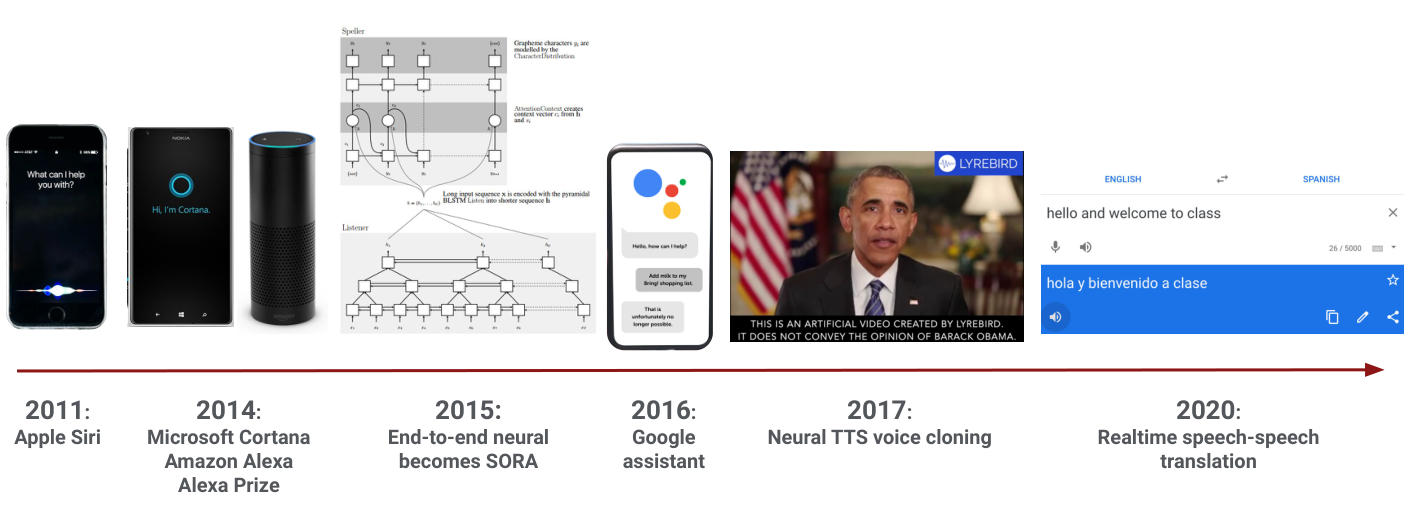
\includegraphics[width=\textwidth,height=0.82\textheight,keepaspectratio]{assets/New-Lecture-TTS/cs224s_2024_lec1/slide_04.png}
\end{frame}

% --- Source: Stanford CS224S, 224s.24.lec1.pdf, slide 5 ---
% \begin{frame}{Voice AI in the public eye (I)}
%   \centering
%   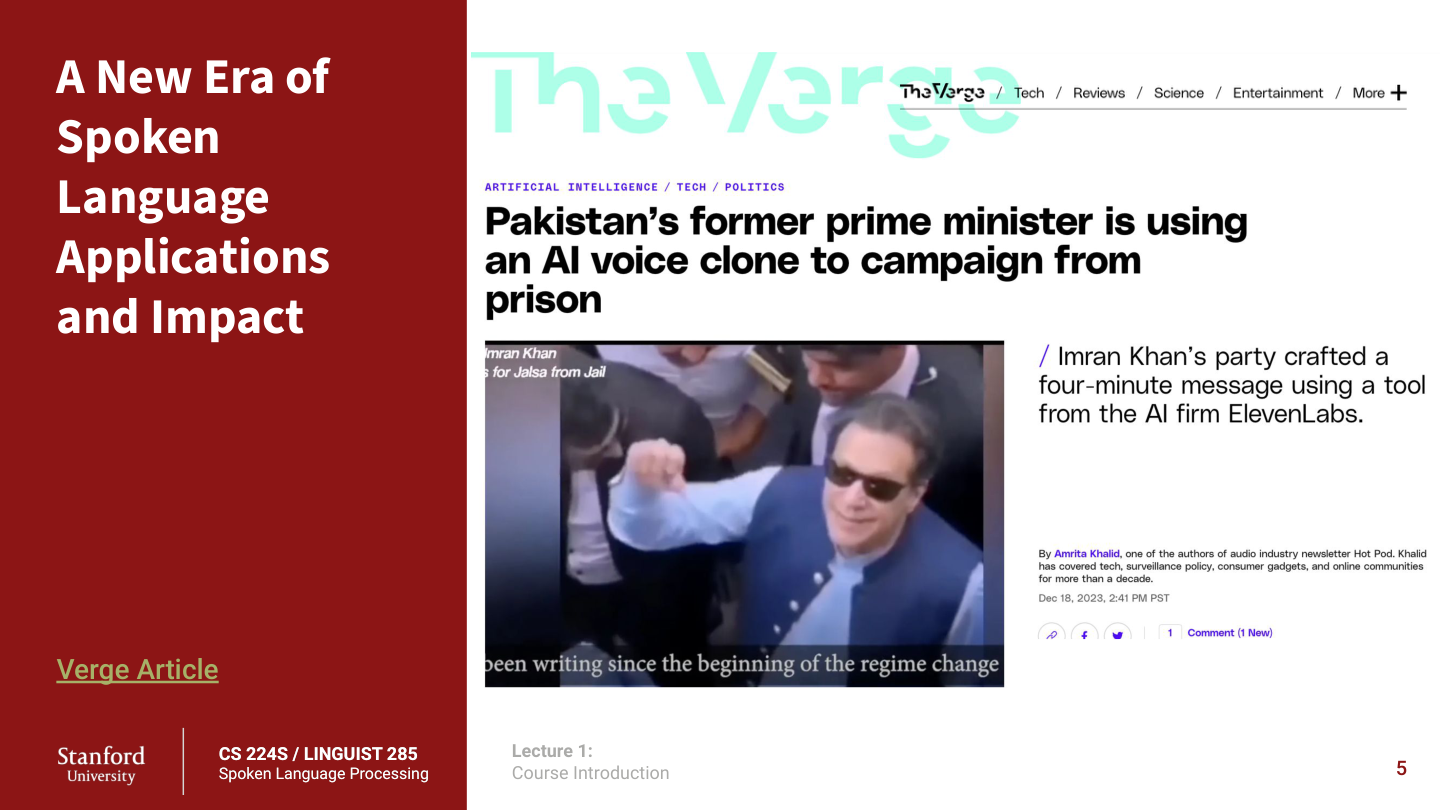
\includegraphics[width=\textwidth,height=0.82\textheight,keepaspectratio]{assets/New-Lecture-TTS/cs224s_2024_lec1/slide_05.png}
%   \slideimgsource{Stanford CS224S, Lecture 1 (2024 Spring), slide 5 (Verge article).}
% \end{frame}


% --- Source: Stanford CS224S, 224s.24.lec1.pdf, slide 24 ---
% \begin{frame}{Why conversational speech is harder}
%   \begin{itemize}
%     \item Utterances are often \textbf{under-specified without context}---prosody and phrasing disambiguate intent.
%     \item TTS must eventually convey that context implicitly through timing, emphasis, and intonation.
%   \end{itemize}
%   \centering
%   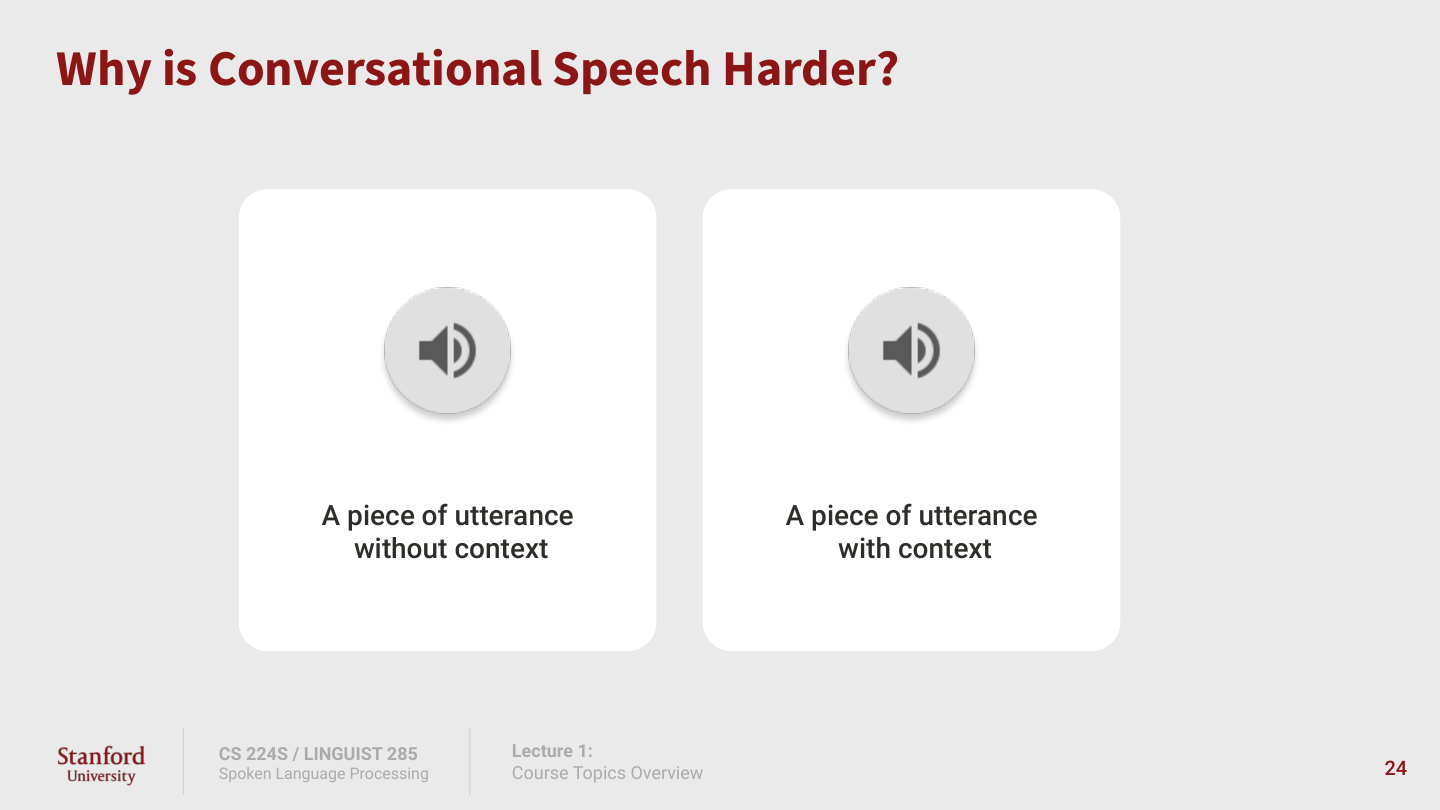
\includegraphics[width=\textwidth,height=0.68\textheight,keepaspectratio]{assets/New-Lecture-TTS/cs224s_2024_lec1/slide_24.png}
%   \slideimgsource{Stanford CS224S, Lecture 1 (2024 Spring), slide 24.}
% \end{frame}

% % --- Source: Stanford CS224S, 224s.24.lec1.pdf, slide 25 ---
% \begin{frame}{Human vs.\ machine speech recognition errors}
%   \centering
%   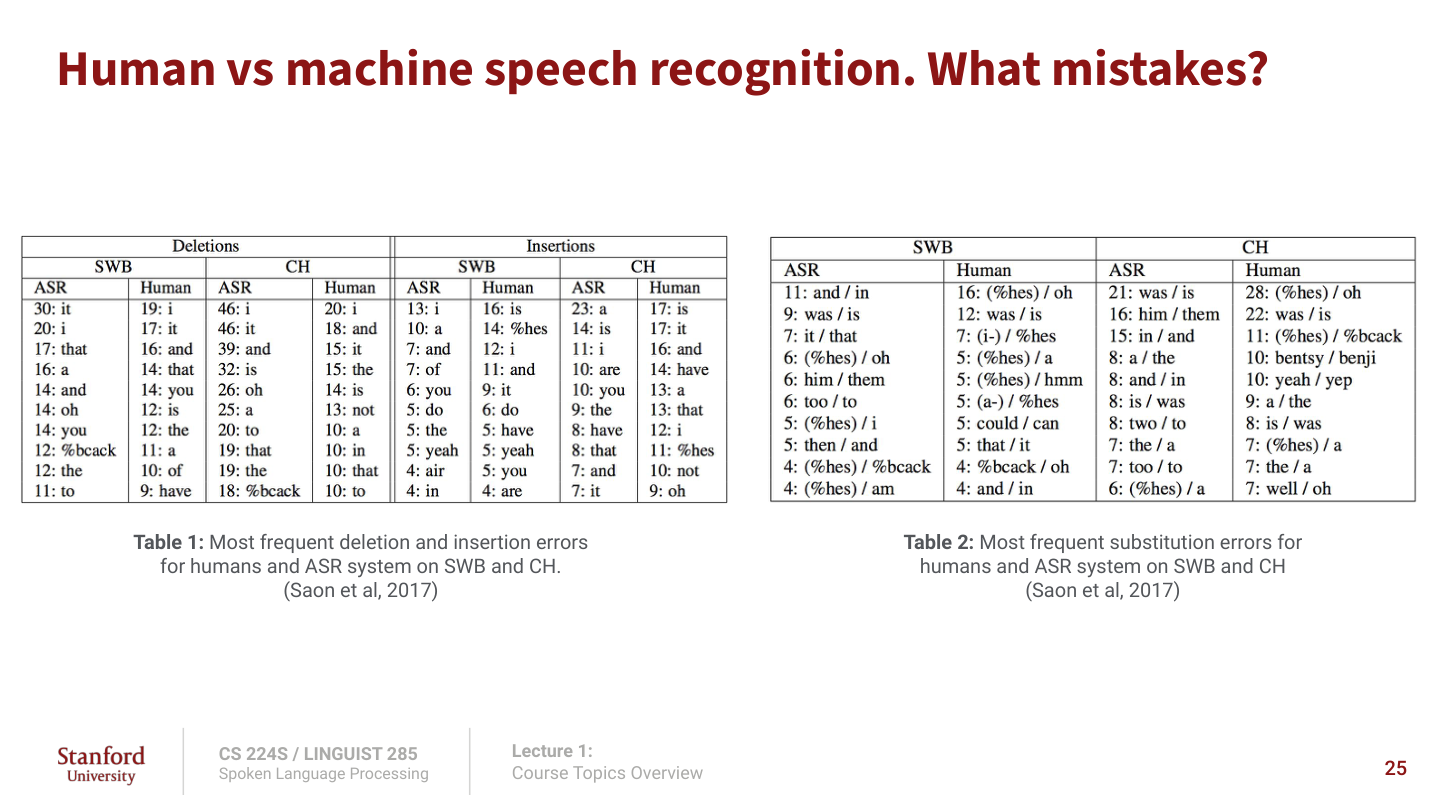
\includegraphics[width=\textwidth,height=0.82\textheight,keepaspectratio]{assets/New-Lecture-TTS/cs224s_2024_lec1/slide_25.png}
%   \slideimgsource{Stanford CS224S, Lecture 1 (2024 Spring), slide 25 (SWB/CH error analysis).}
% \end{frame}

% % --- Source: Stanford CS224S, 224s.24.lec1.pdf, slide 26 ---
% \begin{frame}{Why accents are hard}
%   \begin{itemize}
%     \item The same word in isolation vs.\ in context illustrates how \textbf{coarticulation} and accent shift pronunciations.
%     \item TTS and ASR both struggle when training data under-represent a dialect or L2 accent.
%   \end{itemize}
%   \centering
%   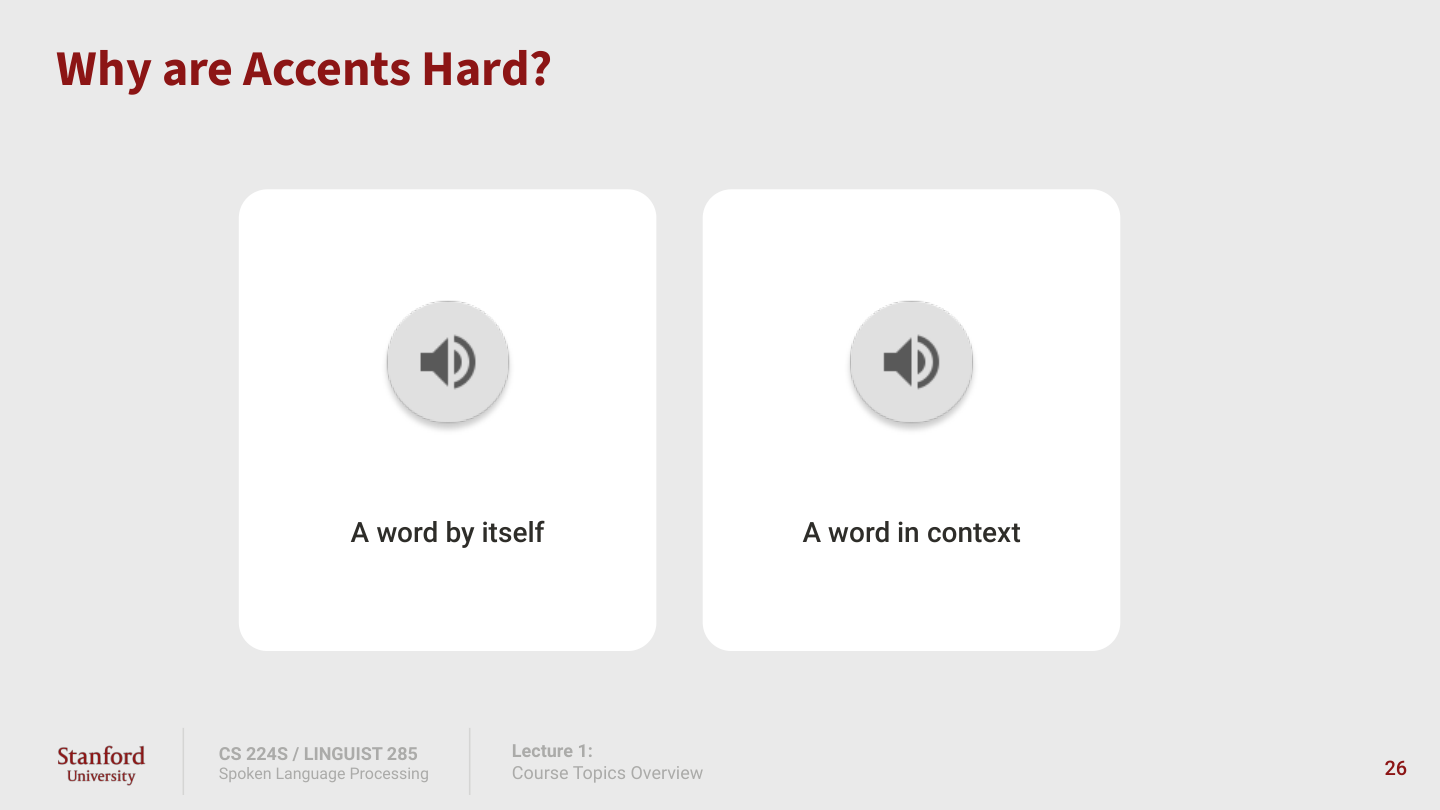
\includegraphics[width=\textwidth,height=0.68\textheight,keepaspectratio]{assets/New-Lecture-TTS/cs224s_2024_lec1/slide_26.png}
%   \slideimgsource{Stanford CS224S, Lecture 1 (2024 Spring), slide 26.}
% \end{frame}

% % --- Source: Stanford CS224S, 224s.24.lec1.pdf, slide 27 ---
% \begin{frame}{Is speech recognition solved?}
%   \centering
%   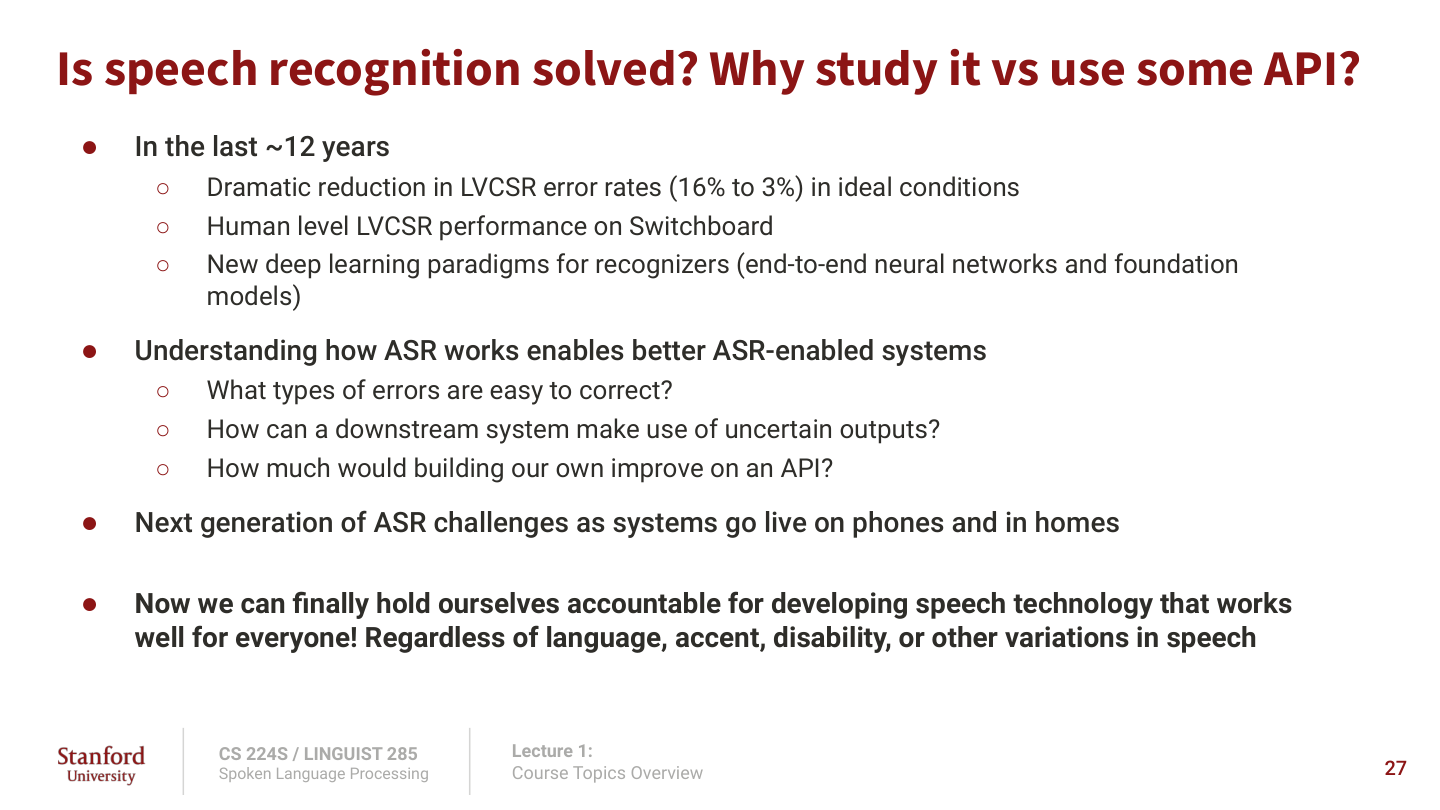
\includegraphics[width=\textwidth,height=0.82\textheight,keepaspectratio]{assets/New-Lecture-TTS/cs224s_2024_lec1/slide_27.png}
%   \slideimgsource{Stanford CS224S, Lecture 1 (2024 Spring), slide 27.}
% \end{frame}

% % --- Source: Stanford CS224S, 224s.24.lec1.pdf, slide 28 ---
% \begin{frame}{ASR design intuition (feeds the full spoken stack)}
%   \begin{itemize}
%     \item Classic view: build a statistical speech-to-words model from \textbf{large transcribed corpora}.
%     \item TTS is the \textbf{inverse problem}---words to speech---but shares front-end and robustness concerns.
%   \end{itemize}
%   \centering
%   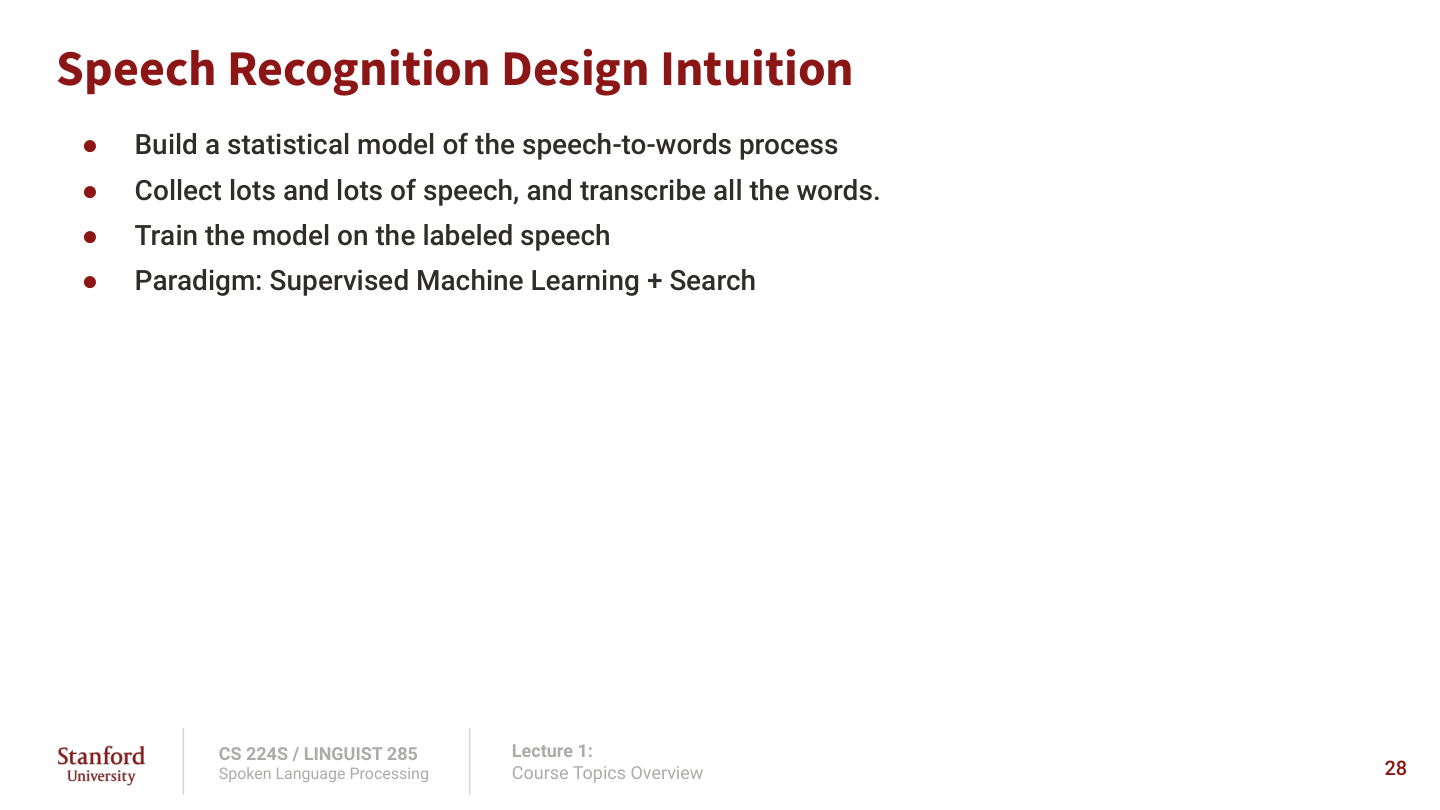
\includegraphics[width=\textwidth,height=0.65\textheight,keepaspectratio]{assets/New-Lecture-TTS/cs224s_2024_lec1/slide_28.png}
%   \slideimgsource{Stanford CS224S, Lecture 1 (2024 Spring), slide 28.}
% \end{frame}

% --- Source: CS224S, Lecture 1, slide 22 ---
\begin{frame}{Snapshot: Task Oriented Dialogue Systems}
  \centering
  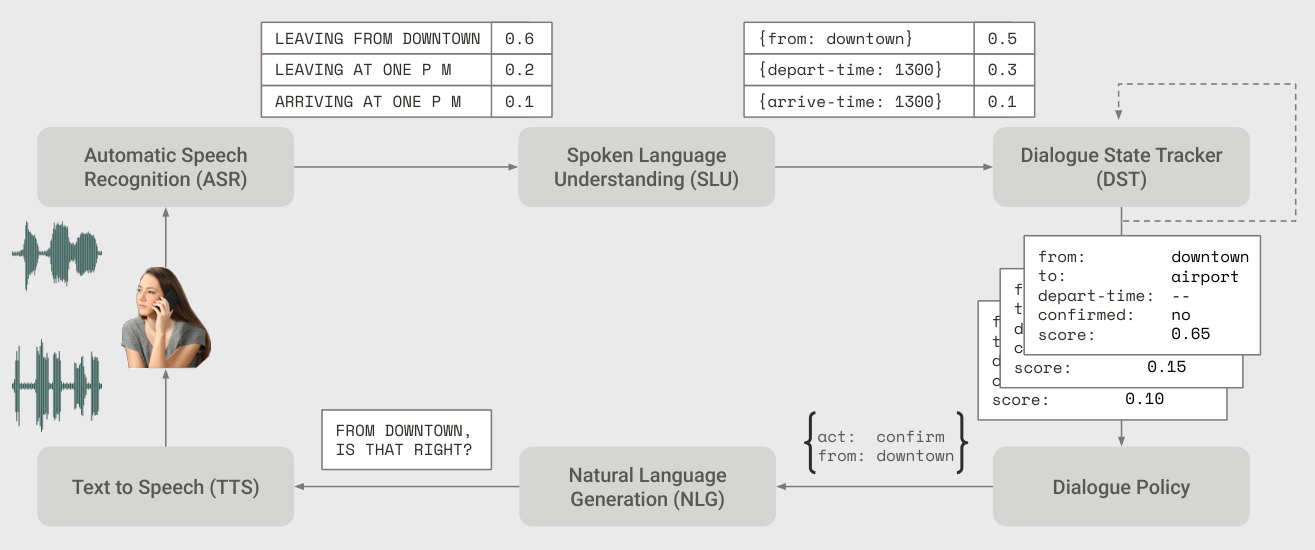
\includegraphics[width=0.92\textwidth,height=0.58\textheight,keepaspectratio]{assets/New-Lecture-TTS/cs224s_compound_ai_pipeline.png}
  \captionof{figure}{Architecture of dialogue-state system for task-oriented dialogue (William et al, 2016)}
\end{frame}


% --- Source: Stanford CS224S, 224s.24.lec1.pdf, slides 29--31 ---
\begin{frame}{What is Text-to-Speech (TTS)?}
  \begin{itemize}
    \item \textbf{What:} Produce speech from a text input (\textbf{Input:} text, optionally with speaker, language, style, or acoustic prompt; \textbf{Output:} waveform or codec tokens perceived as speech).
    \item \textbf{Applications:} 
      \begin{itemize}
        \item Accessibility (screen readers, assistive tech)
        \item Personal Assistants (Apple Siri, Microsoft Cortana, Google Assistant)
        \item Navigation, games, announcements/voice-overs, audiobooks, dubbing, AR/VR
        \item Synthetic data for ASR
      \end{itemize}     
    \end{itemize}
\end{frame}

\begin{frame}{What is Text-to-Speech (TTS)?}
  \begin{itemize}
    \item \textbf{Core difficulty:} Many-to-many mapping --- the same text admits many natural realizations (prosody, rate, emphasis).
    \item \textbf{New variation:} Voice cloning --- TTS systems that mimic particular speakers with minimal training data.
  \end{itemize}
\end{frame}

% --- Source: Stanford CS224S, 224s.24.lec1.pdf, slide 30 ---
\begin{frame}{TTS Overview}
  \begin{itemize}
    \item Collect lots of speech (5--50 hours) from one speaker, transcribe very carefully, all the syllables and phones and whatnot.
    \item Rapid recent progress in neural approaches.
    \item Modern systems are DNN-based, understandable, but not yet fully emotive.
    \item No longer require extensive data from a single speaker to make a TTS voice for them.
  \end{itemize}
\end{frame}

\begin{frame}{TTS: Definitions}
  \begin{itemize}
    \item \textbf{Codec:} A coder/decoder system that encodes analog speech signals into a digitized, discrete compressed representation for compression.
    \item The discrete symbols a codec produces as its compressed form can serve as \textbf{discrete codes} for language modeling.
    \item A codec typically consists of:
      \begin{itemize}
        \item An \textbf{encoder} (\textit{e.g.}, convnets) that downsamples speech into an embedding,
        \item A \textbf{quantizer} that converts the embedding into a series of discrete tokens,
        \item A \textbf{decoder} (\textit{e.g.}, convnets) that upsamples the tokens/embedding back into a (lossy) reconstructed waveform.
      \end{itemize}
  \end{itemize}
\end{frame}

% % --- Source: Stanford CS224S, 224s.24.lec1.pdf, slide 6 ---
% \begin{frame}{Voice AI in the public eye (II)}
%   \centering
%   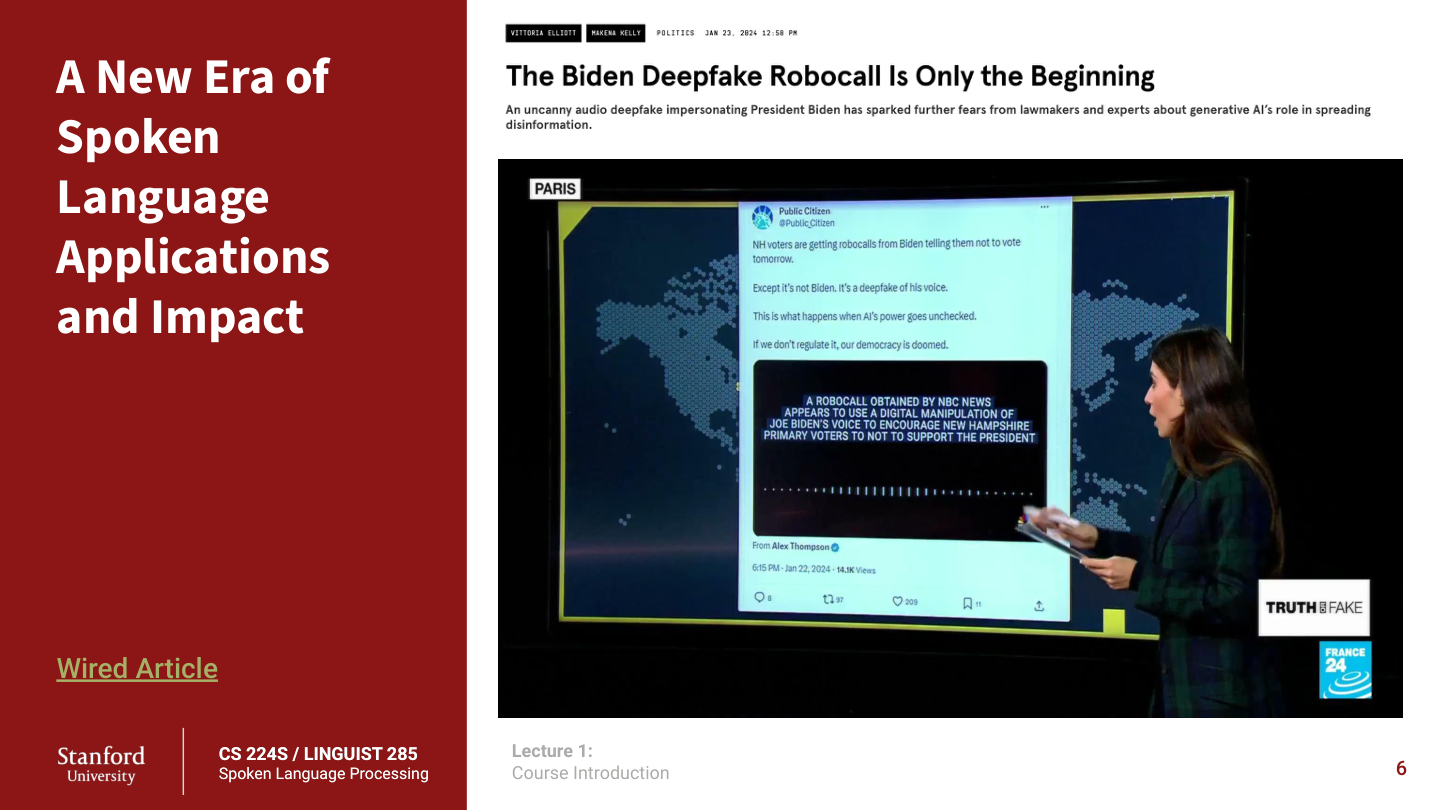
\includegraphics[width=\textwidth,height=0.82\textheight,keepaspectratio]{assets/New-Lecture-TTS/cs224s_2024_lec1/slide_06.png}
%   \slideimgsource{Stanford CS224S, Lecture 1 (2024 Spring), slide 6 (Wired article).}
% \end{frame}

% % --- Source: Stanford CS224S, 224s.24.lec1.pdf, slide 7 ---
% \begin{frame}{Voice AI in the public eye (III)}
%   \centering
%   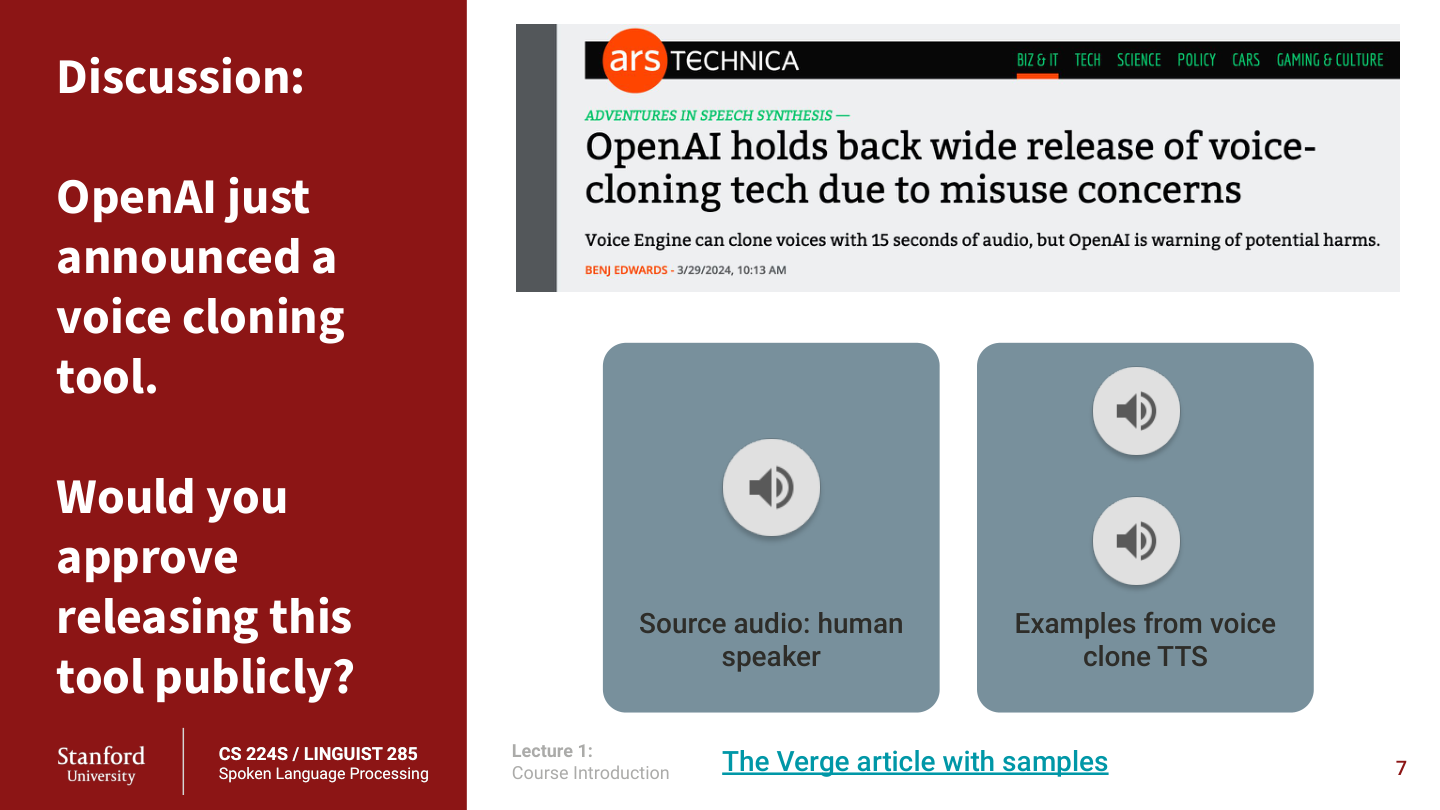
\includegraphics[width=\textwidth,height=0.82\textheight,keepaspectratio]{assets/New-Lecture-TTS/cs224s_2024_lec1/slide_07.png}
%   \slideimgsource{Stanford CS224S, Lecture 1 (2024 Spring), slide 7 (The Verge, with samples).}
% \end{frame}

\begin{frame}{TTS: Modular Pipeline}
  \begin{enumerate}
    \item \textbf{Text analysis} --- normalization, tokenization, G2P
    \item \textbf{Acoustic model} --- mel, latents, or codec codes over time
    \item \textbf{Vocoder / decoder} --- waveform or neural codec inversion
  \end{enumerate}
  \centering
  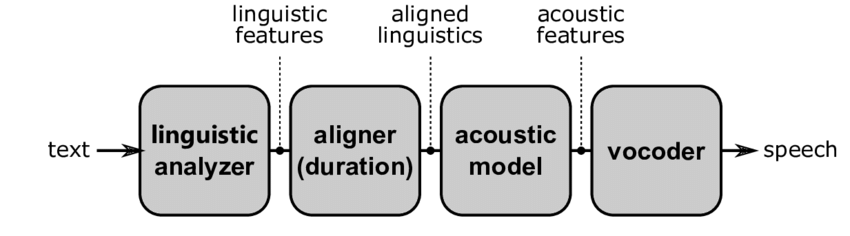
\includegraphics[width=0.86\textwidth,keepaspectratio]{images/audio-nlp/tts_pipeline.png}
\end{frame}

% --- Source: TTS Lecture Material Generation Request (report body: Historical Taxonomy) ---
\begin{frame}{Three eras of text-to-speech}
  \begin{itemize}
    \item \textbf{Pre-2016:} concatenative unit selection and statistical parametric (HMM/GMM) synthesis.
    \item \textbf{2016--2021:} neural end-to-end models (Tacotron~2, WaveNet vocoders, FastSpeech, Glow-TTS, VITS).
    \item \textbf{2022--present:} diffusion, flow matching, and \textbf{foundation audio} models (VALL-E, Voicebox) with zero-shot cloning and in-context control.
    \item Each era targets bottlenecks of the previous one: flexibility, fidelity, latency, then controllability at scale.
  \end{itemize}
\end{frame}

% --- Source: TTS Lecture Material Generation Request (report table); CMU intro / SPSS (Works cited 6--7) ---
\begin{frame}{Three eras of text-to-speech}
  \footnotesize
  {\scriptsize
  \begin{tabular}{@{}llll@{}}
    \hline
    \textbf{Era} & \textbf{Technology} & \textbf{Strength} & \textbf{Bottleneck} \\
    \hline
    Concatenative & Unit / diphone selection & Local timbre & Huge DB; brittle joins \\
    Statistical (SPSS) & HMM / GMM vocoder params & Small footprint; adaptation & Muffled, averaged sound \\
    Neural (E2E) & Tacotron~2 + neural vocoder & High fidelity; simpler stack & Slow AR inference \\
    Foundation & VALL-E, Voicebox & Zero-shot; in-context learning & Data scale; misuse risk \\
    \hline
  \end{tabular}
  }
\end{frame}
